%PDFTexify
\RequirePackage{atbegshi}
%\documentclass[envcountsect]{beamer}
\documentclass[xcolor=dvipsnames]{beamer}
\usepackage{tikz}
\usetikzlibrary{calc}
\usepackage{beamerthemesplit}
\usepackage[utf8]{inputenc}
\usepackage{pgf,pgfarrows,pgfnodes,pgfautomata,pgfheaps}
\usepackage{subfigure,graphicx}
\usepackage{amsmath,amssymb}
\usepackage{color}
\usepackage{rotating}
\usepackage{pgfplots}
\usepackage{textpos}
\usepackage{xspace}
\usepackage{dsfont}
\usepackage{ifthen}
\usepackage{array}
\usepackage{multirow}
\usepackage{eurosym}
\usepackage{etoolbox}
\usepackage{calc}
\usepackage[export]{adjustbox}
\usepackage{xargs}
\usepackage{fancyvrb}
\newboolean{printlogo}
\usepackage{enumerate}
\usepackage{paralist}
\usepackage{graphicx}
\usepackage{multicol}
\usepackage{tikz}
\usepackage{lipsum}
\usepackage{listings}
%\usecolortheme{klu}

%----------------------------------------------------------------------------

%----------------------------------------------------------------------------
%\newcommand{\vortragstitel}{}
\newcommand{\currentsemester}{June 17, 2020}
\newcommand{\lecturetitle}{Polyhedral Study of the \\ Weighted Linear Ordering Problem}%title
\newcommand{\lecturesubtitle}{Polyhedral Study of the wLOP}%subtitle
\newcommand{\lecturer}{Jessica Hautz, Philipp Hungerländer, \textbf{Tobias Lechner}, \\ Kerstin Maier, Peter Rescher} % Autoren
\newcommand{\speaker}{Tobias Lechner}%Speaker
\newcommand{\email}{toblechner@edu.aau.at} %email
\newcommand{\tocTitle}{Content}%Beschriftung (Titel) der Inhaltsfolien
\newcommand{\refTitle}{References}%Beschriftung Literaturfolien
\setboolean{printlogo}{true}%Logo auf den Folien ein/ausschalten
%----------------------------------------------------------------------------

%----------------------------------------------------------------------------
%Farben
\definecolor{klu}{cmyk}{0.60 0.10 0.00 0.20}
\definecolor{aaublau}{RGB}{31,112,132}
\definecolor{aaublaudunkel}{RGB}{13,83,101}
%----------------------------------------------------------------------------

%input "literatur.bib"
\setbeamertemplate{bibliography item}[literatur.bib]

\newcommand{\rb}[1]{\raisebox{1.5ex}[-1.5ex]{#1}}
\newcommand{\MOD}{\mathop{\text{MOD}}}
\newcommand{\TO}{\Rightarrow}
\newcommand{\DIV}{\mathop{\text{DIV}}}
%\newcommand{\ggt}{\text{ggT}}
\newcommand{\dividesnot}{\!\!\not|}
\newcommand{\R}{\mathds{R}}
\newcommand{\Z}{\mathds{Z}}
\newcommand{\N}{\mathds{N}}
\newcommand{\To}{\rightarrow}
\newcommand{\eps}{\varepsilon}
\newcommand{\set}[1]{\left\{#1\right\}}
\newcommand{\abs}[1]{\left|#1\right|}
\newcommand{\norm}[1]{\left\|#1\right\|}
\newcommand{\I}{\mathcal{I}}
\newcommand{\compl}[1]{\overline{#1}}

\newcommand{\rot}[1]{\textcolor[rgb]{1.00,0.00,0.00}{#1}\xspace}
\newcommand{\blau}[1]{\textcolor[rgb]{0.00,0.00,1.00}{#1}\xspace}
\newcommand{\gruen}[1]{\textcolor[rgb]{0.00,1.00,0.00}{#1}\xspace}
\newcommand{\grau}[1]{\textcolor[rgb]{0.50,0.50,0.50}{#1}\xspace}
\newcommand{\blueColor}{
    \setbeamercolor{title}{fg=aaublaudunkel}
    \setbeamercolor{title}{bg=klu!25}
    \setbeamercolor{frametitle}{bg=klu!25}
    \setbeamercolor{frametitle}{fg=aaublaudunkel}
    \setbeamercolor{structure}{fg=aaublaudunkel}
    %\setbeamercolor{structure}{bg=UniRed}
    \setbeamercolor{block title}{use=structure,fg=aaublaudunkel,bg=klu!25}
	\setbeamercolor{block body}{use=structure,fg=black,bg=klu!10}
}

\newcommand\blfootnote[1]{%
  \begingroup
  \renewcommand\thefootnote{}\footnote{#1}%
  \addtocounter{footnote}{-1}%
  \endgroup
}

\newcommand{\emptypage}{\frame{}}
\newtheorem{satz}{Satz}[section]
\newtheorem{thm}{Theorem}[section]
\newtheorem{kor}{Corollary}[section]
\newtheorem{lem}{Lemma}[section]

\newcounter{bsp}
\newenvironment{bsp}[1][]{\refstepcounter{bsp}\par\medskip\noindent%
   \blau{Beispiel~\thebsp #1:}}{\hfill$\diamond$\medskip}
\numberwithin{bsp}{section}

\renewcommand{\qed}{\hfill$\square$}
\newcommand{\bew}{\underline{Beweis}:~}
\newenvironmentx{beweis}[1][1=\empty]{\ifthenelse{\equal{#1}{\empty}}{\par\medskip\noindent\bew}
{\par\medskip\noindent\underline{Beweis} (#1):~}}{\qed}

\newenvironment{slide}[1]{\blueColor\begin{frame}\frametitle{#1}}{\end{frame}}
\newenvironment{mslide}[1]{\blueColor\begin{frame}[allowframebreaks]\frametitle{#1}}{\end{frame}}
\newenvironment{redslide}[1]{\redColor\begin{frame}\frametitle{#1}}{\end{frame}}
\newenvironment{redmslide}[1]{\redColor\begin{frame}[allowframebreaks]\frametitle{#1}}{\end{frame}}

\usetheme{Boadilla}
\usecolortheme{seahorse}
\setbeamertemplate{blocks}[rounded][shadow=true]
\setbeamertemplate{caption}[numbered]
\setbeamertemplate{navigation symbols}{}

\setbeamertemplate{footline}
{
  \leavevmode%
  \hbox{%
  \begin{beamercolorbox}[wd=.7\paperwidth,ht=2.25ex,dp=1ex,left]{author in head/foot}%
    \usebeamerfont{author in head/foot}\hspace{1cm}{\speaker}\hspace{1cm}\lecturesubtitle%\insertshortauthor
  \end{beamercolorbox}%
  \begin{beamercolorbox}[wd=.3\paperwidth,ht=2.25ex,dp=1ex,right]{title in head/foot}%
    \usebeamerfont{title in head/foot}\currentsemester%\insertshorttitle
    \hspace*{3em}
    \insertframenumber{}\hspace*{1em}%/ \inserttotalframenumber
  \end{beamercolorbox}}%
  \vskip0pt%
}
\setbeamertemplate{headline}[text line]{
  \begin{beamercolorbox}[wd=\paperwidth,ht=5ex,dp=4ex]{}
    \insertsectionnavigationhorizontal{\textwidth}{}{}
%    \raisebox{-10pt}{\includegraphics[width=15mm]{UNI_KLU_Logo_cmyk}}\vskip2pt
%    \hskip-1pt\rule{\paperwidth}{0.3pt}
  \end{beamercolorbox}
}

\ifthenelse{\boolean{printlogo}}{
\addtobeamertemplate{frametitle}{}{%
\begin{textblock*}{100mm}(.85\textwidth,-0.75cm)

\includegraphics[width=2cm]{aaulogo}
\end{textblock*}
}
}{}

\setbeamertemplate{theorems}[numbered]
\setbeamertemplate{caption}[numbered]
\numberwithin{figure}{section}

\title[\lecturetitle]{\lecturetitle}
\author{\phantom{Yg}\lecturer\phantom{Yg}}
\titlegraphic{
\includegraphics[width=26mm]{fig_aau-logo-department.pdf}}
\institute{Alpen-Adria-Universität Klagenfurt}
\date{June 17, 2020}

\begin{document}

\blueColor
\begin{frame}[plain]
\titlepage
\end{frame}

\begin{frame}[plain]
\frametitle{Contents}
\linespread{1.4}
\tableofcontents
\end{frame}


\section{Introduction and Recap}

\subsection{Definitions}

%\frame%<presentation>
% {\fontsize{11.5pt}{9pt}\selectfont
\begin{frame}[plain]
   \frametitle{Contents}
   \linespread{1.1}
   \tableofcontents[currentsubsection]
\end{frame}



\begin{frame}
	\begin{block}{Halfspace}
		A set $H \subseteq \mathbb{R}^{n}$ is called halfspace if it can be written as \begin{equation*}
		H=\{ x \in \mathbb{R}^{n}\mid a^{T}x \leq b \}
		\end{equation*} for some $a\in \mathbb{R}^{n}$,\ $b \in \mathbb{R}$.
	\end{block}

\begin{block}{Polyhedron}
	The intersection of finitely many halfspaces is called polyhedron. A polyhedron can be written as 
	\begin{equation*}
	P=\{ x \in \mathbb{R}^{n} \mid Ax \leq b\}
	\end{equation*}  with $A\in \mathbb{R}^{m\times n}$,\ $b \in \mathbb{R}^{m}$.
\end{block}
\end{frame}

\begin{frame}
\begin{block}{Polytope}
	A bounded polyhedron is called polytope. Each polytope $P \subset \mathbb{R}^{n}$ can be written as the convex hull of finitely many points.
\end{block}

\begin{block}{Dimension of a polyhedron}
	The dimension of a polyhedron $P \subset \mathbb{R}^{n}$ equals k if the maximal number of affinely independent points in $P$ is $k+1$.
\end{block}
\end{frame}

\begin{frame}
	\begin{block}{Valid inequality}
		An inequality $a^{T}x \leq b, a, x \in \mathbb{R}^{n}, b \in \mathbb{R}$ is called valid for a polyhedron $P \subset \mathbb{R}^{n}$ if $P \subset \{ x \in \mathbb{R}^{n}\mid a^{T}x \leq b\}$.
	\end{block}

\begin{block}{Supporting inequality}
	A valid inequality supports the polyhedron $P$ if there exist points $x \in P$ with $a^{T}x = b$.
\end{block}
	
\begin{block}{Proper inequality}
	A valid inequality is called proper if $P \not \subset \{ x \in \mathbb{R}^{n}\mid a^{T}x = b\}$.
\end{block}
\end{frame}

\begin{frame}
	\begin{block}{Face}
		A subset $F$ of a polyhedron $P$ is called face of $P$ if there exists a valid inequality $a^{T}x \leq b,\ a, x \in \mathbb{R}^{n},\ b \in \mathbb{R}$ such that $F= \{x\in P\mid a^{T}x = b\}$ holds.
	\end{block}
	
	\begin{block}{Facet}
		A proper nonempty face $F$ of a polyhedron $P$ is called facet if 
		\begin{equation*}
		dim(F) = dim(P)-1.
		\end{equation*}
	\end{block}
\end{frame}


\subsection{Example of a polytope}
%\frame%<presentation>
%{\fontsize{11.5pt}{9pt}\selectfont
%	\frametitle{Contents}\tableofcontents[currentsubsection]}

\begin{frame}[plain]
	\frametitle{Contents}
	\linespread{1.1}
	\tableofcontents[currentsubsection]
\end{frame}

\begin{frame}
	\frametitle{Example}
	Polytope in form of a dodekahedron:
	\begin{center}
		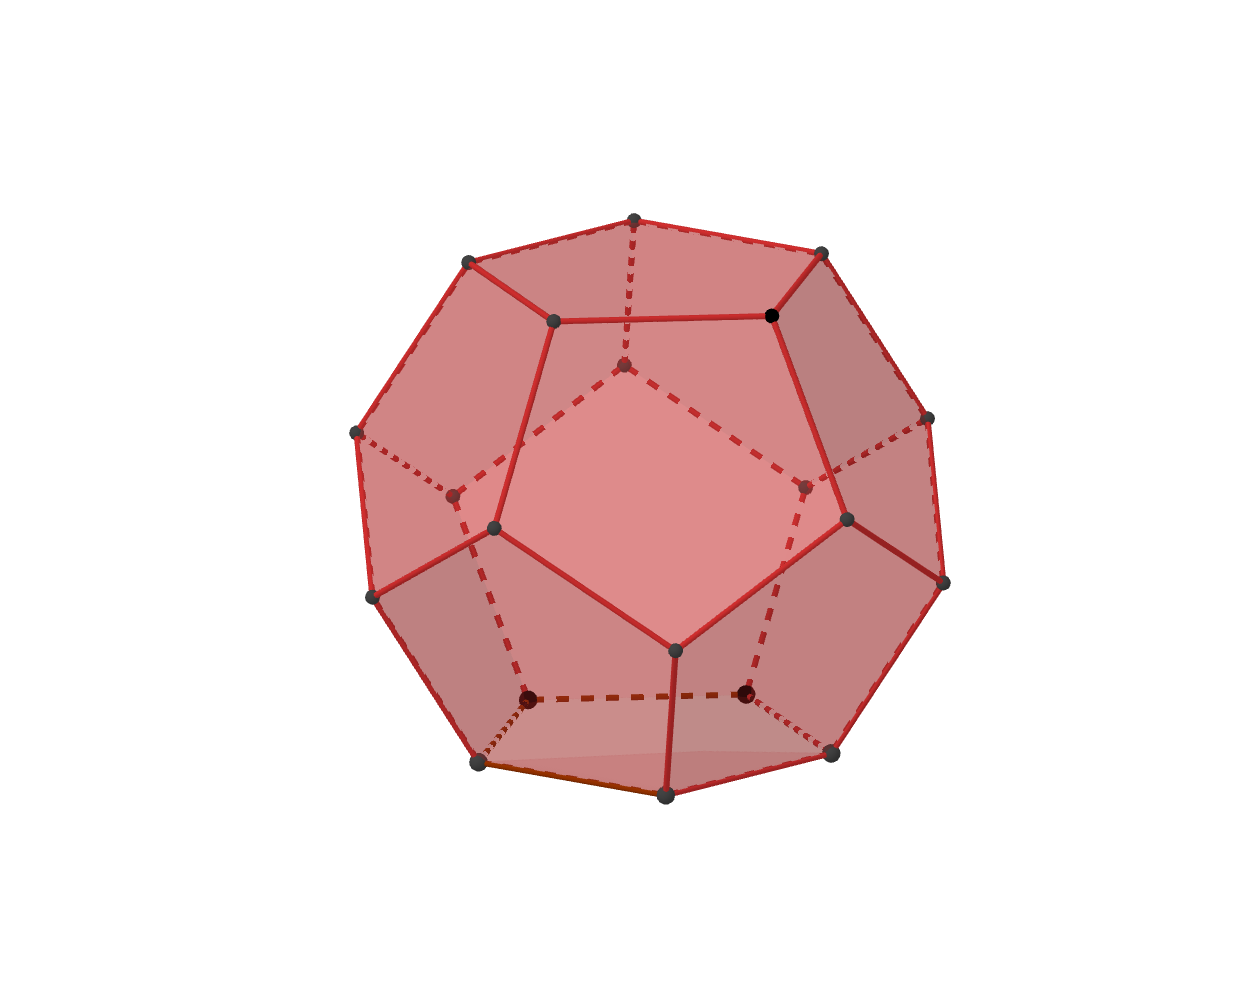
\includegraphics[scale=0.3]{DodeNormal.PNG}
	\end{center} 
\end{frame}

\begin{frame}
	\frametitle{Example}
	Visualization of a halfspace and face with dimension 0:
	\begin{center}
		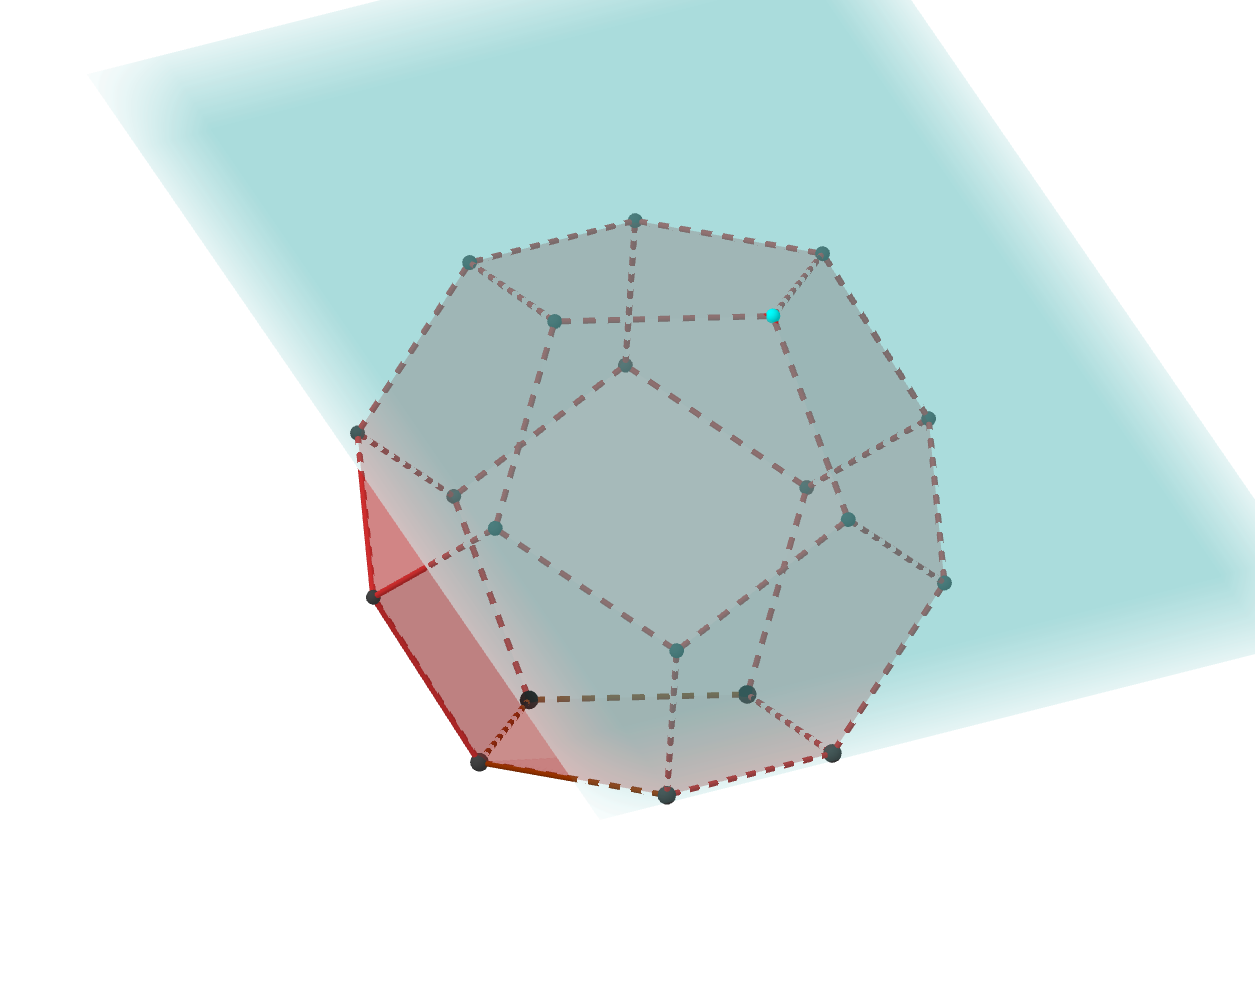
\includegraphics[scale=0.3]{DodeHalfspacepunkt.PNG}
	\end{center} 
\end{frame}

\begin{frame}
	\frametitle{Example}
	Visualization of a halfspace and face with dimension 1:
	\begin{center}
		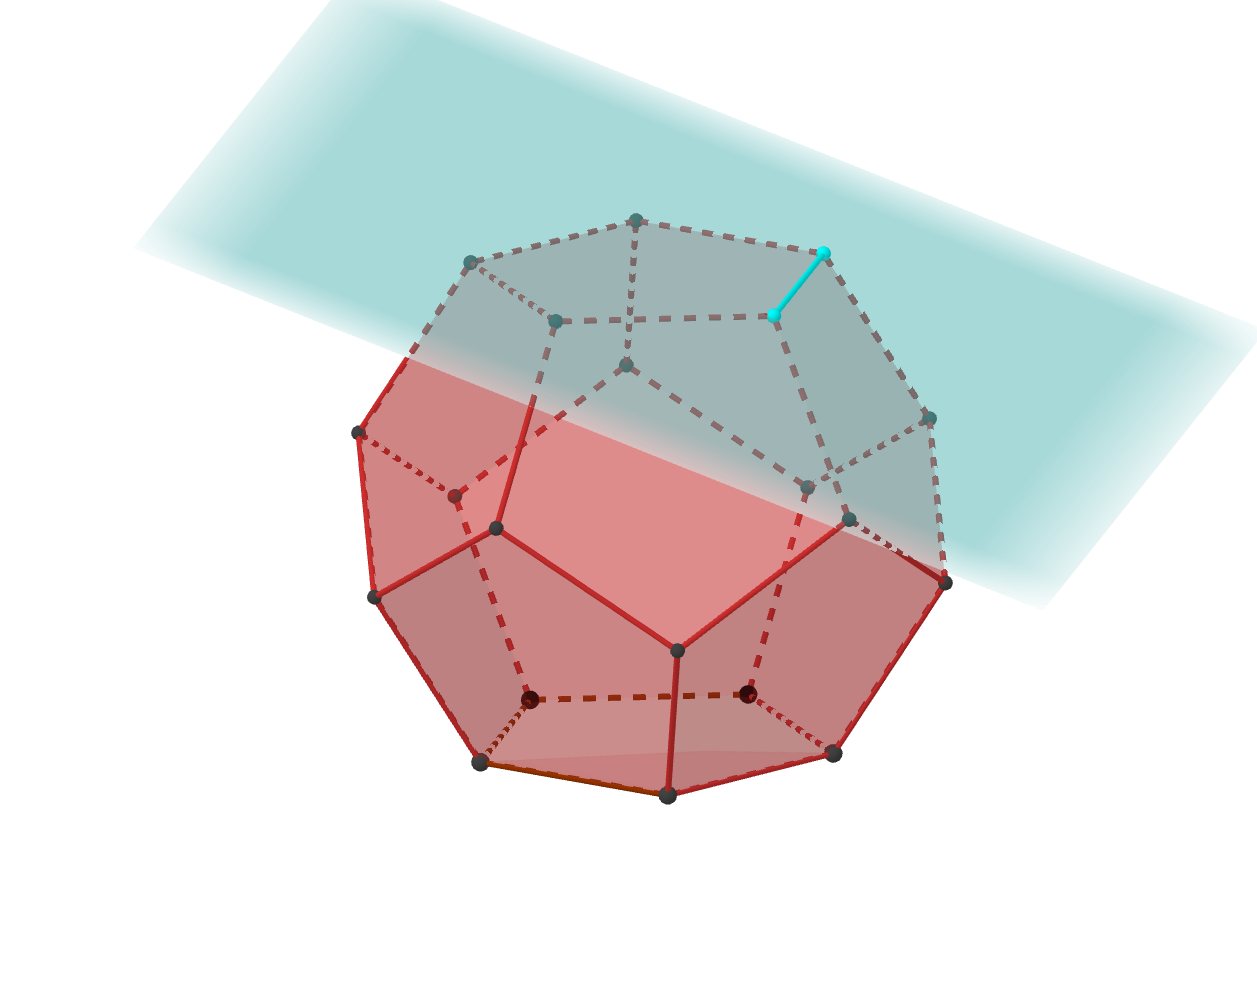
\includegraphics[scale=0.3]{DodeHalfspacelinie.PNG}
	\end{center} 
\end{frame}

\begin{frame}
	\frametitle{Example}
	Visualization of a halfspace and face with dimension 2 (facet):
	\begin{center}
		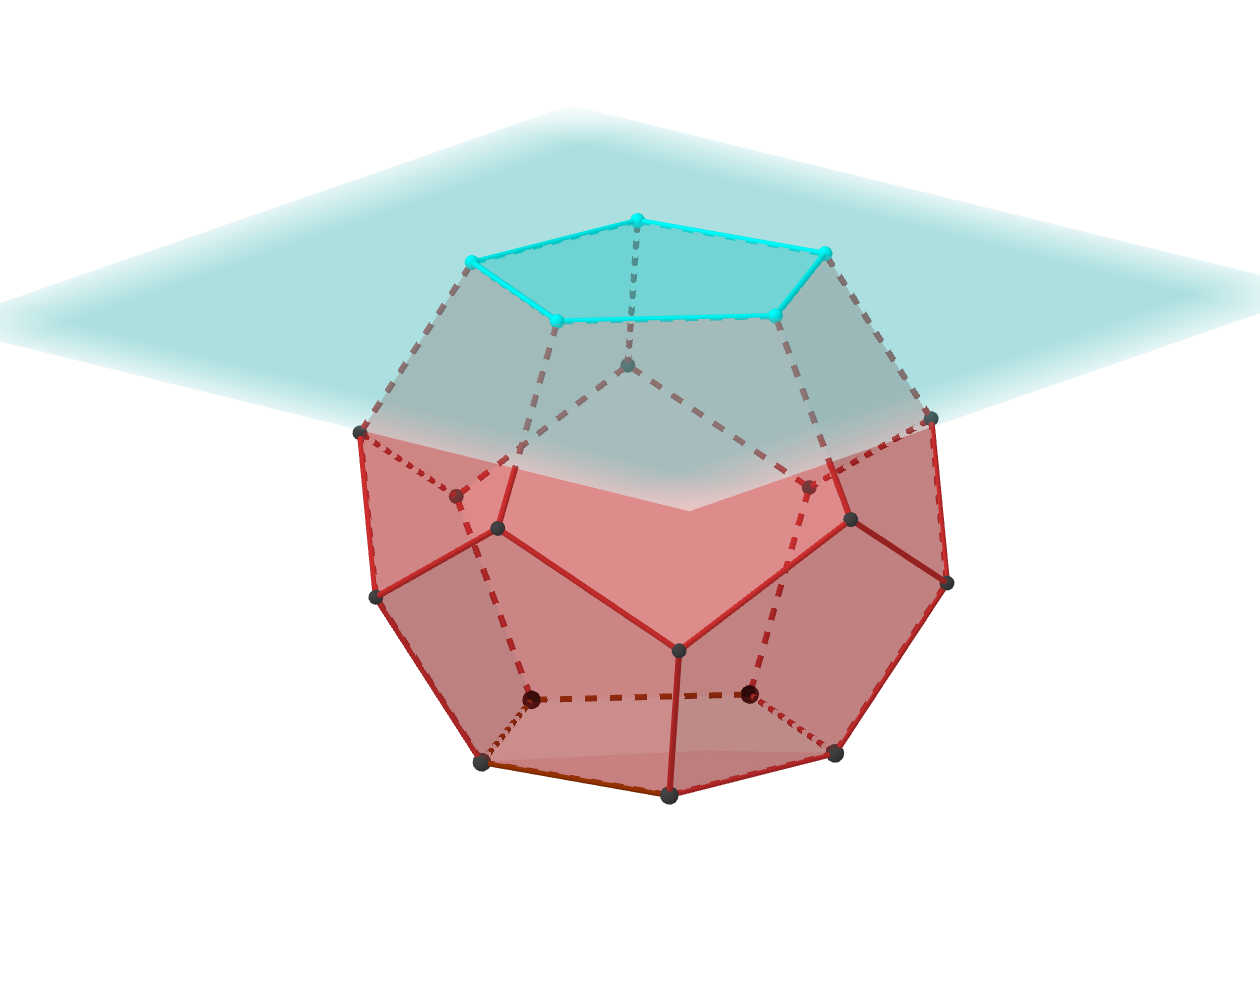
\includegraphics[scale=0.3]{DodeHalfspaceobenblau.PNG}
	\end{center} 
\end{frame}

\begin{frame}
	\begin{block}{Summary of this example polyhedral study}
		\begin{itemize}
			\item Points in $\mathbb{R}^{3}$
			\item Bounded polyhedron $\rightarrow$ polytope
			\item 12 faces of dimension 2 (facets)
			\item 30 faces of dimension 1 (edges)
			\item 20 faces of dimension 0 (corners)
		\end{itemize}
	\end{block}
\end{frame}

\subsection{Meaning of equality constraints}

%\frame%<presentation>
% {\fontsize{11.5pt}{9pt}\selectfont
\begin{frame}[plain]
	\frametitle{Contents}
	\linespread{1.1}
	\tableofcontents[currentsubsection]
\end{frame}

\begin{frame}
	\frametitle{Special type of constraints}
	\begin{block}{Equality constraints}
		A special case of constraints of a polyhedron occurs, when it is defined by two halfspaces of the form 
		\begin{center}
			$H_{1}=\{ x \in \mathbb{R}^{n}\mid a^{T}x \leq b \}$
			
			\vspace{10 pt}
			
			$H_{2}=\{ x \in \mathbb{R}^{n}\mid a^{T}x \geq b \}$
		\end{center}
		
		In this case these two constraints can be combined to one equality constraint:
		
		\begin{center}
			$H=\{ x \in \mathbb{R}^{n}\mid a^{T}x = b \}$
			
			\vspace{10 pt}
			
		\end{center}
		
	\end{block}
\end{frame}

\begin{frame}
	\frametitle{Special type of constraints}
	\begin{block}{Consequences of equality constraints}
		Let the polytope P be defined as $P=\{x \in \mathbb{R}^{n}\mid A^{T}x \leq b \}$ and let $A^{=} $ and $b^{=}$ be the matrix and vector corresponding to the equality constraints. Then
		
		\begin{equation*}
		dim(P) = n - rank(A^{=},b^{=}).
		\end{equation*}
		
		\vspace{10 pt}
	\end{block}
\end{frame}

\begin{frame}
	\frametitle{Example of equality constraints in $\mathbb{R}^{3}$}
	Visualization of one equality constraint:
	\begin{center}
		
\includegraphics[scale=0.17]{ebene1.PNG}
	\end{center} 
\end{frame}

\begin{frame}
	\frametitle{Example of equality constraints in $\mathbb{R}^{3}$}
	Visualization of two linearly independent equality constraints:
	\begin{center}
		
\includegraphics[scale=0.17]{ebene2linie.PNG}
	\end{center} 
\end{frame}

\begin{frame}
	\frametitle{Example of equality constraints in $\mathbb{R}^{3}$}
	Visualization of three linearly independent equality constraints:
	\begin{center}
		
\includegraphics[scale=0.17]{ebene3punkt.PNG}
	\end{center} 
\end{frame}

\begin{frame}
	\frametitle{Example of equality constraints in $\mathbb{R}^{3}$}
	Visualization of three linearly dependent equality constraints:
	\begin{center}
		
\includegraphics[scale=0.17]{ebene3linie.PNG}
	\end{center} 
\end{frame}

\section{Study of the wLOP-polytope}

\subsection{First analysis of the wLOP polytope}

%\frame%<presentation>
% {\fontsize{11.5pt}{9pt}\selectfont
\begin{frame}[plain]
	\frametitle{Contents}
	\linespread{1.1}
	\tableofcontents[currentsubsection]
\end{frame}

\begin{frame}
	\frametitle{Weighted Linear Ordering Problem (wLOP)}
	
	\begin{description} \item [\textcolor{klu}{Given:}] $n$ one-dimensional objects $[n]=\{1, \ldots,n\}$,  \\ individual object weights $w_{1},\ldots,w_{n}$ and \\ pairwise weights
		$w_{ij}\geq 0, i,j\in [n], i\neq j$.\\\vspace*{0.5cm}
		
		\item[\textcolor{klu}{Goal:}] Find permutation $\pi$ of maximum weight:
	\end{description}
	\begin{equation*}
	\max_{\pi \in \Pi_n} \sum_{\substack{i,j \in [n]\\\pi(i)<\pi(j)}}w_{ij}d_{ij}^{\pi}.
	\end{equation*}
	\begin{align*}
	d_{ij}^{\pi} = \begin{cases} \frac{w_i+w_j}{2} + \sum\limits_{\substack{k \in [n]\\\pi(i) <
			\pi(k) < \pi(j)}}w_k,\qquad  & \pi(i) < \pi(j),\\
	0, & \text{otherwise}.
	\end{cases}
	\end{align*}
\end{frame}

\begin{frame}
	\frametitle{Integer Linear Program (ILP)}
	\begin{block}{Binary Ordering Variables}
		$$ x_{ikj} = \begin{cases} 1, & \text{$i$ is located before $k$ and $k$ is located before $j$},\\
		& \hphantom{} i, j, k \in [n], \quad i \neq j \neq k \neq i,\\
		0, & \text{otherwise}. \\
		\end{cases} $$
	\end{block}
	\begin{block}{Constraints}
		\vspace{-0.5cm}
		\begin{align}
		&x_{ikj} + x_{jki} + x_{ijk} + x_{kji} + x_{jik} + x_{kij} = 1, \quad i, j, k \in [n]\label{equ:permutation} \\
		&x_{ijk} + x_{ikj} + x_{kij} - x_{ij\ell} - x_{i\ell j} - x_{\ell ij} = 0, \quad i, j, k, \ell \in [n]\label{equ:cycle}
		\end{align}
	\end{block}
	$$ x_{mij} + x_{imj} + x_{ijm} = \begin{cases} 1, & \text{if node $i$ is located before node $j$},\\
	& \hphantom{} i, j, m \in [n], \quad i \neq j \neq m\\
	0, & \text{otherwise}. \\
	\end{cases} $$
\end{frame}

\begin{frame}
	\frametitle{ILP}
	\begin{block}{Distance Variables}
		%$$d_{ij} = (\frac{w_i+w_j}{2}) + \sum_{\substack{k \in [n]\\ i \neq j \neq k }}{x_{ikj} w_k}$$.
		\begin{align*}d_{ij} = \left(\frac{w_i+w_j}{2}\right)\frac{\sum_{\substack{k \in [n]\\ i \neq k \neq j }}\left(x_{kij} + x_{ikj} + x_{ijk}\right)}{n - 2} + \sum_{\substack{k \in [n]\\ i \neq k \neq j }}{x_{ikj} w_k}, \, i,j \in [n], i\neq j.\end{align*}
	\end{block}
	\begin{block}{ILP-Formulation}
		\vspace{-0.5cm}
		\begin{align*}
		\max \quad&\sum_{\substack{i,j \in [n]}} w_{ij}d_{ij}.\\
		\text{s. t.} \quad& \eqref{equ:permutation}, \eqref{equ:cycle},\\
		&x_{ikj} \in \{0,1\}, \ i,k,j \in [n], \ i\neq k \neq j \neq i.
		\end{align*}
	\end{block}
\end{frame}


\begin{frame}{Analysis of the wLOP polytope}
	\begin{block}{Basic characteristics}
		\begin{itemize}
			\item Polytope in $\{0,1\}^{n(n-1)(n-2)}$.
			\item Only equality constraints.
		\end{itemize}
	\end{block}
\end{frame}

\subsection{Visualization of 0/1-polytopes}

%\frame%<presentation>
% {\fontsize{11.5pt}{9pt}\selectfont
\begin{frame}[plain]
	\frametitle{Contents}
	\linespread{1.1}
	\tableofcontents[currentsubsection]
\end{frame}

\begin{frame}
	\frametitle{0/1-polytope of dimension 1}
	\begin{center}
		\begin{tikzpicture}
		\filldraw [gray] (0,0) circle (2pt) node[below left] {(0)};
		\filldraw [gray] (2,0) circle (2pt) node[below right] {(1)};
		%\node[below right, outer sep=1pt] (2,0) {(1)};
		\draw (0,0) -- (2,0);
		
		\end{tikzpicture}
	\end{center}
\end{frame}

\begin{frame}
	\frametitle{0/1-polytope of dimension 2}
	\begin{center}
		\begin{tikzpicture}
		\filldraw [gray] (0,0) circle (2pt) node[below left] {(0,0)};
		\filldraw [gray] (0,2) circle (2pt) node[above left] {(0,1)};
		\filldraw [gray] (2,0) circle (2pt) node[below right] {(1,0)};
		\filldraw [gray] (2,2) circle (2pt) node[above right] {(1,1)};
		\draw (0,0) -- (0,2);
		\draw (0,0) -- (2,0);
		\draw (0,2) -- (2,2);
		\draw (2,0) -- (2,2);
		\end{tikzpicture}
	\end{center}
\end{frame}

\begin{frame}
	\frametitle{0/1-polytope of dimension 3}
	\begin{center}
		\begin{tikzpicture}
		\filldraw [gray] (0,0) circle (2pt) node[below left] {\small(0,0,0)};
		\filldraw [gray] (0,2) circle (2pt) node[left] {\small(0,1,0)};
		\filldraw [gray] (2,0) circle (2pt) node[below right] {\small(1,0,0)};
		\filldraw [gray] (2,2) circle (2pt) node[right] {\small(1,1,0)};
		\filldraw [gray] (1,1) circle (2pt) node[left] {\small(0,0,1)};
		\filldraw [gray] (1,3) circle (2pt) node[above left] {\small(0,1,1)};
		\filldraw [gray] (3,1) circle (2pt) node[right] {\small(1,0,1)};
		\filldraw [gray] (3,3) circle (2pt) node[above right] {\small(1,1,1)};
		\draw (0,0) -- (0,2);
		\draw (0,0) -- (2,0);
		\draw (0,2) -- (2,2);
		\draw (2,0) -- (2,2);
		\draw (1,1) -- (1,3);
		\draw (1,1) -- (3,1);
		\draw (1,3) -- (3,3);
		\draw (3,1) -- (3,3);
		\draw (0,0) -- (1,1);
		\draw (0,2) -- (1,3);
		\draw (2,0) -- (3,1);
		\draw (2,2) -- (3,3);
		\end{tikzpicture}
	\end{center}
\end{frame}

\begin{frame}
	\frametitle{0/1-polytope of dimension 4}
	\begin{center}
		\begin{tikzpicture}
		\filldraw [gray] (0,0) circle (2pt) node[below left] {\scriptsize(0,0,0,0)};
		\filldraw [gray] (0,2) circle (2pt) node[left] {\scriptsize(0,1,0,0)};
		\filldraw [gray] (2,0) circle (2pt) node[below right] {\scriptsize(1,0,0,0)};
		\filldraw [gray] (2,2) circle (2pt) node[right] {\scriptsize(1,1,0,0)};
		\filldraw [gray] (1,1) circle (2pt) node[left] {\scriptsize(0,0,1,0)};
		\filldraw [gray] (1,3) circle (2pt) node[left] {\scriptsize(0,1,1,0)};
		\filldraw [gray] (3,1) circle (2pt) node[right] {\scriptsize(1,0,1,0)};
		\filldraw [gray] (3,3) circle (2pt) node[right] {\scriptsize(1,1,1,0)};
		
		\filldraw [gray] (-0.5,0.5) circle (2pt) node[left] {\scriptsize(0,0,0,1)};
		\filldraw [gray] (-0.5,2.5) circle (2pt) node[left] {\scriptsize(0,1,0,1)};
		\filldraw [gray] (1.5,0.5) circle (2pt) node[right] {\scriptsize(1,0,0,1)};
		\filldraw [gray] (1.5,2.5) circle (2pt) node[right] {\scriptsize(1,1,0,1)};
		\filldraw [gray] (0.5,1.5) circle (2pt) node[left] {\scriptsize(0,0,1,1)};
		\filldraw [gray] (0.5,3.5) circle (2pt) node[above left] {\scriptsize(0,1,1,1)};
		\filldraw [gray] (2.5,1.5) circle (2pt) node[right] {\scriptsize(1,0,1,1)};
		\filldraw [gray] (2.5,3.5) circle (2pt) node[above right] {\scriptsize(1,1,1,1)};
		
		\draw (0,0) -- (0,2);
		\draw (0,0) -- (2,0);
		\draw (0,2) -- (2,2);
		\draw (2,0) -- (2,2);
		\draw (1,1) -- (1,3);
		\draw (1,1) -- (3,1);
		\draw (1,3) -- (3,3);
		\draw (3,1) -- (3,3);
		\draw (0,0) -- (1,1);
		\draw (0,2) -- (1,3);
		\draw (2,0) -- (3,1);
		\draw (2,2) -- (3,3);
		
		\draw (-0.5,0.5) -- (-0.5,2.5);
		\draw (-0.5,0.5) -- (1.5,0.5);
		\draw (-0.5,2.5) -- (1.5,2.5);
		\draw (1.5,0.5) -- (1.5,2.5);
		\draw (0.5,1.5) -- (0.5,3.5);
		\draw (0.5,1.5) -- (2.5,1.5);
		\draw (0.5,3.5) -- (2.5,3.5);
		\draw (2.5,1.5) -- (2.5,3.5);
		\draw (-0.5,0.5) -- (0.5,1.5);
		\draw (-0.5,2.5) -- (0.5,3.5);
		\draw (1.5,0.5) -- (2.5,1.5);
		\draw (1.5,2.5) -- (2.5,3.5);
		
		\draw (0,0) -- (-0.5,0.5);
		\draw (0,2) -- (-0.5,2.5);
		\draw (2,0) -- (1.5,0.5);
		\draw (2,2) -- (1.5,2.5);
		\draw (1,1) -- (0.5,1.5);
		\draw (1,3) -- (0.5,3.5);
		\draw (3,1) -- (2.5,1.5);
		\draw (3,3) -- (2.5,3.5);
		\end{tikzpicture}
	\end{center}
\end{frame}

\subsection{Dimension of the wLOP polytope}

\subsubsection{Redundancy of constraints}
%\frame%<presentation>
% {\fontsize{11.5pt}{9pt}\selectfont
\begin{frame}[plain]
	\frametitle{Contents}
	\linespread{1.1}
	\tableofcontents[currentsubsection]
\end{frame}

\begin{frame}{Dimension of the wLOP polytope}
	We already know a way to determine the dimension of a polytope:
	
	\begin{block}{Consequences of equality constraints}
		Let the polytope P be defined as $P=\{x \in \mathbb{R}^{n}\mid A^{T}x \leq b \}$ and let $A^{=} $ and $b^{=}$ be the matrix and vector corresponding to the equality constraints. Then
		
		\begin{equation*}
		dim(P) = n - rank(A^{=},b^{=}).
		\end{equation*}
		
		\vspace{10 pt}
	\end{block}

	In our case we already know the value of $n$, therefore it remains to determine $rank(A^{=},b^{=})$.
\end{frame}

\begin{frame}{Dimension of the wLOP polytope}	
	\begin{block}{Constraints}
		\vspace{-0.5cm}
		\begin{align*}
		&x_{ikj} + x_{jki} + x_{ijk} + x_{kji} + x_{jik} + x_{kij} = 1, \quad i, j, k \in [n] &(*)\\
		&x_{ijk} + x_{ikj} + x_{kij} - x_{ij\ell} - x_{i\ell j} - x_{\ell ij} = 0, \quad i, j, k, \ell \in [n] &(**)
		\end{align*}
	\end{block}
	\vspace{10 pt}
    To determine $rank(A^{=},b^{=})$ we need to evaluate how many constraints are linearly independent.
\end{frame}

\begin{frame}{Dimension of the wLOP polytope}
	\begin{block}{Important characteristics of the constraints}
		\begin{itemize}
			\item Only one constraint is necessary in $(*)$.
			\item There are cases of two linearly dependent constraints in $(**$).
			\item There are cases of three linearly dependent constraints in $(**)$.
			\item There are cases of six linearly dependent constraints in $(**)$.
		\end{itemize}
	\end{block}
\end{frame}

\begin{frame}{Only one constraint is necessary in $(*)$}
	\begin{block}{Lemma 1}
		One constraints of the form 
		
		\begin{center}
			$x_{ikj} + x_{jki} + x_{ijk} + x_{kji} + x_{jik} + x_{kij} = 1, \quad i, j, k \in [n]$
		\end{center} 
		
		is sufficient to construct every other constraint in $(*)$ with the help of the constraints in $(**)$.
	\end{block}
	
	\begin{block}{Proof}
		The constraints in $(**)$ can be rewritten in the form 

		\begin{center}
			$x_{ijk} + x_{ikj} + x_{kij} =  x_{ij\ell} + x_{i\ell j} + x_{\ell ij}, \quad i, j, k, \ell \in [n]$
		\end{center}
		
		and every constraint in $(*)$ can be constructed by according substitutions.
	\end{block}
\end{frame}

\begin{frame}{Symmetry of constraints in $(**)$}
	\begin{block}{Lemma 2}
		For $i,j,k,\ell \in [n]$ the constraints
		\begin{align*}
		x_{ijk} + x_{ikj} + x_{kij} - x_{ij\ell} - x_{i\ell j} - x_{\ell ij} &= 0 \\
		x_{ij\ell} + x_{i\ell j} + x_{\ell ij} - x_{ijk} - x_{ikj} - x_{kij} &= 0
		\end{align*} 
		
		are equivalent.
	\end{block}
	
	\begin{block}{Proof}
		Multiply the first constraint by $-1$ to obtain the second constraint.
	\end{block}
\end{frame}

\begin{frame}{Transitivity of constraints in $(**)$}
	\begin{block}{Lemma 3}
		For $i,j,k,\ell,m \in [n]$ the following constraints are linearly dependent:
		\vspace{-5 pt}
		\begin{align*}
		x_{ijk} + x_{ikj} + x_{kij} \hspace{1 pt} - x_{ij\ell} \hspace{3 pt} - x_{i\ell j} \hspace{2 pt} - x_{\ell ij} \hspace{3 pt} &= 0, \\
		x_{ijk} + x_{ikj} + x_{kij} - x_{ijm} - x_{imj} - x_{mij} &= 0, \\
		x_{ij\ell} \hspace{1 pt} + x_{i\ell j} + x_{\ell ij} - x_{ijm} - x_{imj} - x_{mij} &= 0,
		\end{align*} 
	\end{block}
	
	\begin{block}{Proof}
		Subtract the first constraint from the second one to obtain the third constraint.
	\end{block}
\end{frame}

\begin{frame}{Linear Dependence of six constraints in $(**)$}
	\begin{block}{Lemma 4}
		For $i,j,k,\ell \in [n]$ the following constraints are linearly dependent:
		\vspace{-5 pt}
		\begin{align*}
		x_{ijk} + x_{ikj} + x_{kij} - x_{ijl}\hspace{1 pt} - x_{ilj}\hspace{2 pt} - x_{lij}\hspace{2 pt} &= 0, \\
		x_{ikj} + x_{ijk} + x_{jik} - x_{ikl} - x_{ilk} - x_{lik} &= 0, \\
		x_{ilj}\hspace{2 pt} + x_{ijl}\hspace{2 pt} + x_{jil}\hspace{2 pt} - x_{ilk} - x_{ikl} - x_{kil} &= 0, \\
		x_{jik} + x_{jki} + x_{kji} - x_{jil}\hspace{2 pt} - x_{jli}\hspace{2 pt} - x_{lji}\hspace{2 pt} &= 0, \\
		x_{kij} + x_{kji} + x_{jki} - x_{kil} - x_{kli} - x_{lki} &= 0, \\
		x_{lij}\hspace{2 pt} + x_{lji}\hspace{2 pt} + x_{jli}\hspace{2 pt} - x_{lik} - x_{lki} - x_{kli} &= 0.
		\end{align*}
	\end{block}
	
	\begin{block}{Proof}
		Add the second and fifth constraint and subtract the first, third and fourth constraint to obtain the last one.
	\end{block}
\end{frame}

\subsubsection{Construction scheme for linearly independent constraints}
%\frame%<presentation>
% {\fontsize{11.5pt}{9pt}\selectfont
\begin{frame}[plain]
	\frametitle{Contents}
	\linespread{1.1}
	\tableofcontents[currentsubsection]
\end{frame}

\begin{frame}[fragile] 
	\frametitle{Constructionscheme}
	\begin{block}{Theorem 1}
		For every given $n>4$ the following subset of constraints contains all constraints of $(**)$ in its span. We define this subset by going through all of the $\frac{n(n-1)(n-2)(n-3)}{2}$ constraints in ascending order.
		\scriptsize
	\begin{lstlisting}
	3(n-1) times: 		n-3 times:		included
				binom{n-3}{2} times:	redundant
	for i in {3, ... , n-1}:
		i times:	i-2 times:		redundant
				n-i-1 times:		included
				binom{n-3}{2} times:	redundant
	
		n-i-1 times: 	n-3 times:		included
				binom{n-3}{2} times:	redundant
	\end{lstlisting}
	\end{block}
	\begin{block}{Proof}
		Show redundancies with Lemmas 1-4. (long)
	\end{block}
\end{frame}

\begin{frame}{Linear independence}
	\begin{block}{Theorem 2}
		The set of constraints defined in the constructionscheme in theorem 1 is linearly independent.
	\end{block}
	
	\begin{block}{Proof}
		Show, that the x-variable of highest order with non-zero coefficient is different in every included constraint.
	\end{block}
\end{frame}

\begin{frame}
	\frametitle{Constraintmatrix for $n=5$}
	\begin{center}
		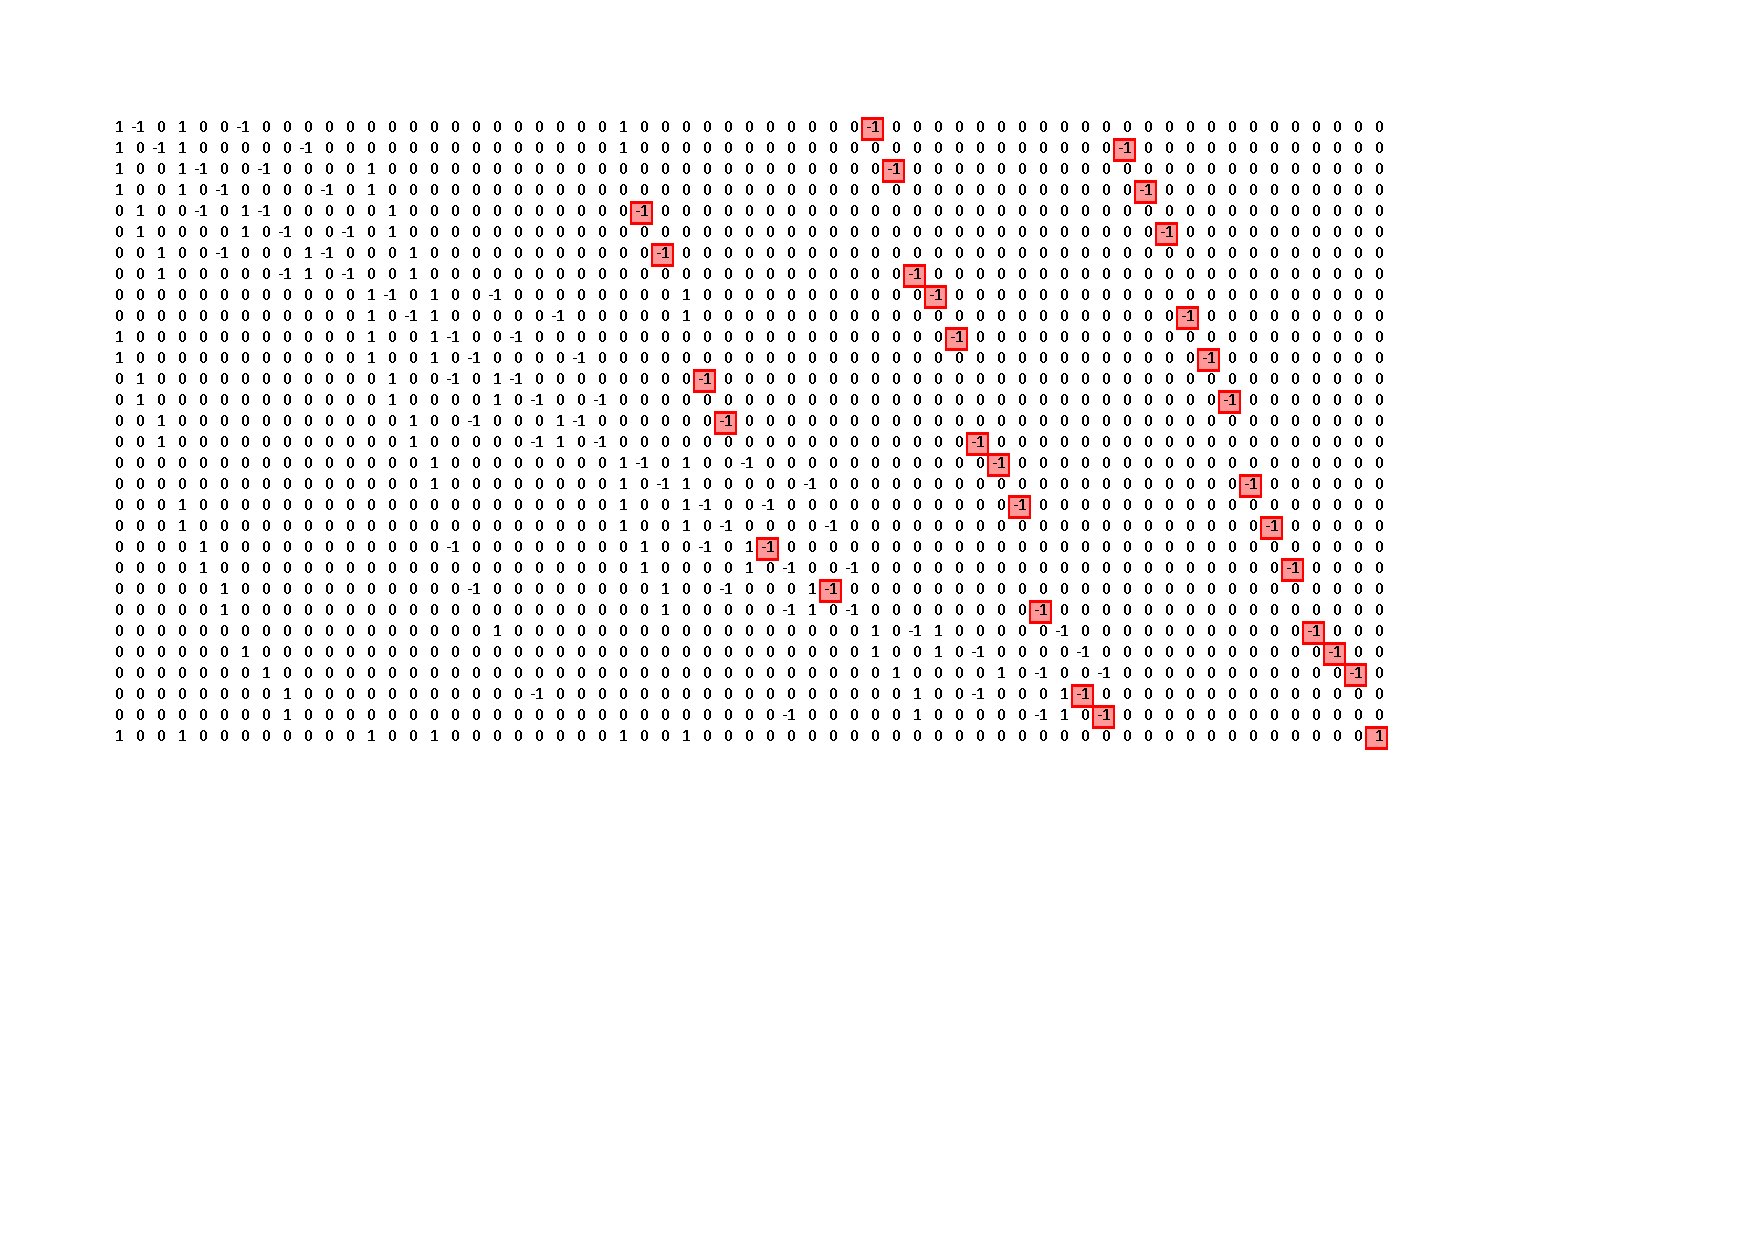
\includegraphics[scale=0.5]{Matrix5rosa_cropped.pdf}
	\end{center} 
\end{frame}

\begin{frame}
	\frametitle{Constraintmatrix for $n=5$}
	\begin{center}
		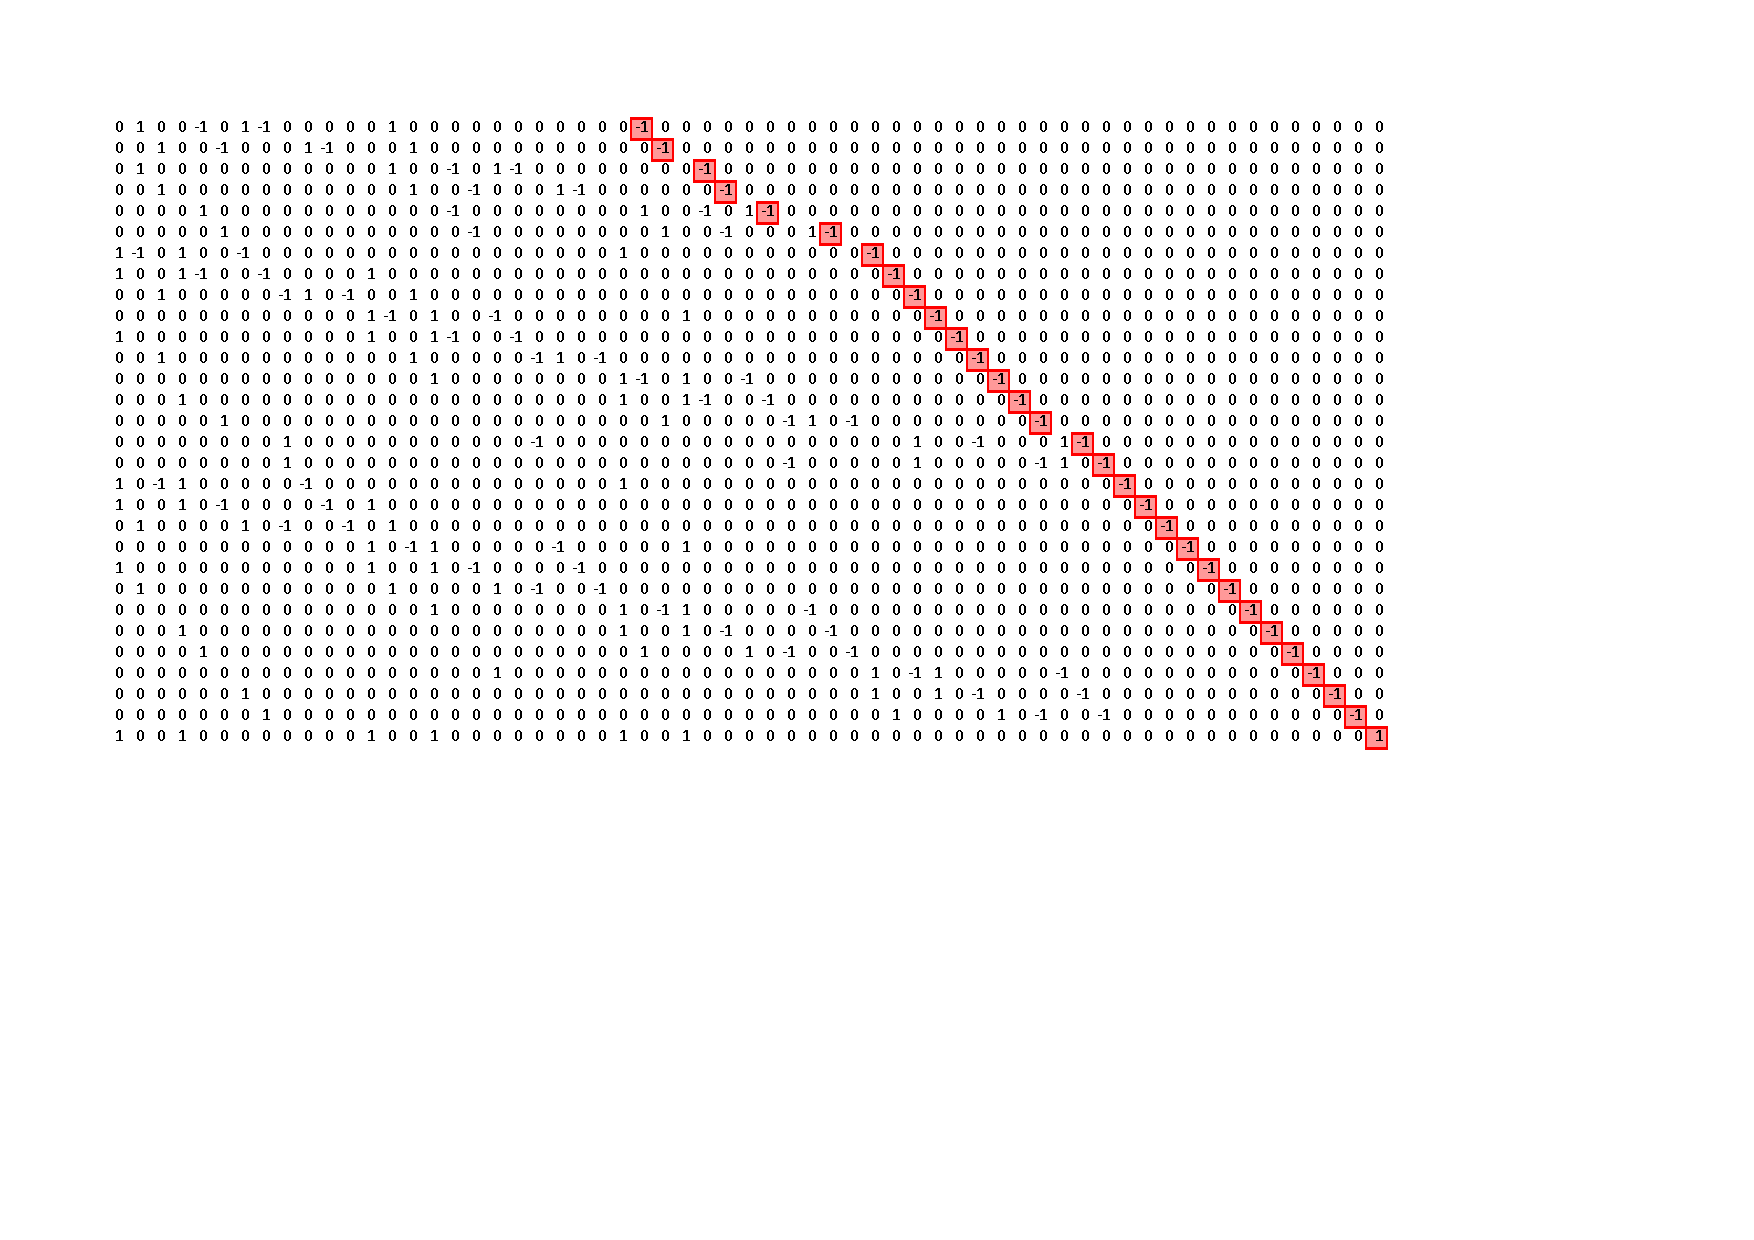
\includegraphics[scale=0.5]{Matrix5rosaDreieck_cropped.pdf}
	\end{center} 
\end{frame}

\begin{frame}{Linear independence}
	\begin{block}{Corollary 1}
		The dimension of the wLOP polytope for a given number of objects $n$ is 
		\vspace{-5 pt}
		\begin{center}
			$\frac{n^3}{3}+ \frac{n^2}{2} + \frac{n}{6}$.
		\end{center}
	\end{block}
	
	\begin{block}{Proof}
		Determine how many constraints are included in the construction scheme and subtract from the number of variables.
	\end{block}
\end{frame}

\section{Conclusion and outlook}

\begin{frame}{Conclusion and outlook}
	\begin{itemize}
		\item We constructed a minimal set of necessary constraints. 
		
		(Before: $n^{4}-5n^{3}+8n^{2}-4n$ constraints, now: $\frac{2}{3}n^3- \frac{5}{2}n^2 + \frac{11}{6}n$.)
		\item The dimension of the wLOP polytope is $\frac{n^3}{3}+ \frac{n^2}{2} + \frac{n}{6}$.
		\item Polyhedra of high dimensions are difficult to visualize/ examine.
		\item Future work: determine facets of the wLOP polytope and study different ILP formulations.
	\end{itemize}
\end{frame}



\begin{frame}[plain]{\titlepage}\end{frame}
\end{document}